\begin{figure}[htbp]
			\centering
			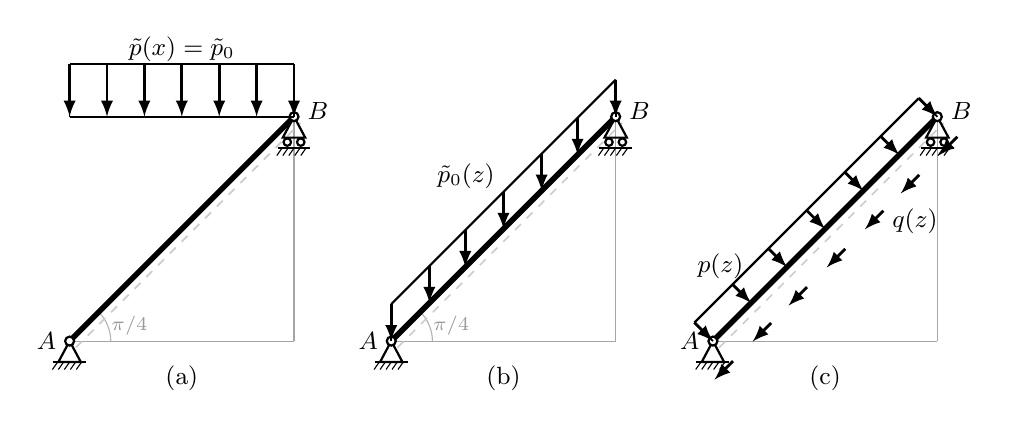
\begin{tikzpicture}[
				scale=0.95,
				>=latex,
				trave/.style={line width=2pt},
				%carico/.style={blue!70!black, line width=1pt},
				carico/.style={line width=1pt},
				%			pcomp/.style={teal!60!black, line width=1pt},
				pcomp/.style={line width=1pt},
				%			qcomp/.style={orange!80!black, line width=1pt},
				qcomp/.style={line width=1pt},
				tratt/.style={gray!70, thin},
				fibre/.style={dashed, gray!40, line width=0.6pt},
				]
				
				% =========================================================
				% PANNELLO (a)
				% =========================================================
				\begin{scope}[xshift=0cm]
					
					% ── Parametri dei vincoli (convenzione C06/C07) ──
					\def\tw{0.15}    % semi-larghezza triangolo
					\def\thR{0.28}   % altezza triangolo
					\def\rn{0.06}    % raggio anellino (perno)
					\def\rw{0.05}    % raggio ruote del carrello
					\def\bw{0.09}    % semi-distanza ruote
					\def\gw{0.22}    % semi-larghezza barra di terra
					\def\hh{0.10}    % profondità del tratteggio del suolo
					
					% ── Linee guida e angolo π/4 ──
					\draw[tratt] (0,0) -- (3,0);
					\draw[tratt] (3,0) -- (3,3);
					
					\draw[gray!60] (0.55,0) arc (0:45:0.55);
					\node[gray!80, font=\scriptsize] at (0.80,0.20) {$\pi/4$};
					
					% ── Trave (con fibra inferiore) ──
					\draw[fibre] (0.0849,-0.0849) -- (3.0849,2.9151);
					\draw[trave] (0,0) -- (3,3);
					
					% ── Cerniera in A=(0,0) (suolo orizzontale) ──
					\draw[thick] (0,0) -- (-\tw,-\thR) -- (\tw,-\thR) -- cycle;
					% barra di terra (alla base del triangolo)
					\draw[thick] (-\gw,-\thR) -- (\gw,-\thR);
					% tratteggio del suolo
					\foreach \x in {-0.16,-0.08,0,0.08,0.16}
					\draw[thin] (\x,-\thR) -- ++(-0.07,-\hh);
					
					% ── Carrello in B=(3,3), asse di scorrimento orizzontale ──
					\draw[thick] (3,3) -- (3-\tw,3-\thR) -- (3+\tw,3-\thR) -- cycle;
					% due ruote (sotto la base del triangolo, tangenti)
					\draw[thick] (3-\bw,3-\thR-\rw-0.01) circle (\rw);
					\draw[thick] (3+\bw,3-\thR-\rw-0.01) circle (\rw);
					% barra di terra (sotto le ruote)
					\draw[thick] (3-\gw,3-\thR-2*\rw-0.04) -- (3+\gw,3-\thR-2*\rw-0.04);
					% tratteggio del suolo
					\foreach \x in {-0.16,-0.08,0,0.08,0.16}
					\draw[thin] (3+\x,3-\thR-2*\rw-0.04) -- ++(-0.07,-\hh);
					
					% ── Anellini (perni) in A e B
					%    disegnati per ultimi per restare in primo piano ──
					\draw[thick, fill=white] (0,0) circle (\rn);
					\draw[thick, fill=white] (3,3) circle (\rn);
					
					% ── Etichette A e B (posizioni originali) ──
					\node[left,  font=\small] at (-0.05, 0.) {$A$};
					\node[right, font=\small] at ( 3.05, 3.08) {$B$};
					
					% ── Carico distribuito p(x) = \tilde{p}_0 ──
					\foreach \px in {0.00, 0.50, 1.00, 1.50, 2.00, 2.50, 3.00}{
						\draw[->, carico] (\px, 3.70) -- (\px, 3);
					}
					\draw[carico, line width=0.8pt]	(0.00, 3.70) -- (3.00, 3.70);
					\draw[carico, line width=0.6pt]	(0.00, 3.70) -- (0.00, 3);
					\draw[carico, line width=0.6pt]	(3.00, 3.70) -- (3.00, 3);
					\draw[carico, line width=0.8pt]	(0.00, 3.0) -- (3.00, 3.0);
					
					\node[font=\small] at (1.50,3.90){$\tilde{p}(x) = \tilde{p}_0$};
					
					% ── Etichetta pannello ──
					\node[font=\small] at (1.5,-0.50) {(a)};
					
				\end{scope}
				
				% =========================================================
				% PANNELLO (b)
				% =========================================================
				\begin{scope}[xshift=4.3cm]
					
					% ── Parametri dei vincoli (convenzione C06/C07) ──
					\def\tw{0.15}    % semi-larghezza triangolo
					\def\thR{0.28}   % altezza triangolo
					\def\rn{0.06}    % raggio anellino (perno)
					\def\rw{0.05}    % raggio ruote del carrello
					\def\bw{0.09}    % semi-distanza ruote
					\def\gw{0.22}    % semi-larghezza barra di terra
					\def\hh{0.10}    % profondità del tratteggio del suolo
					
					% ── Linee guida e angolo π/4 ──
					\draw[tratt] (0,0) -- (3,0);
					\draw[tratt] (3,0) -- (3,3);
					
					\draw[gray!60] (0.55,0) arc (0:45:0.55);
					\node[gray!80, font=\scriptsize] at (0.80,0.20) {$\pi/4$};
					
					% ── Trave (con fibra inferiore) ──
					\draw[fibre] (0.0849,-0.0849) -- (3.0849,2.9151);
					\draw[trave] (0,0) -- (3,3);
					
					% ── Cerniera in A=(0,0) (suolo orizzontale) ──
					\draw[thick] (0,0) -- (-\tw,-\thR) -- (\tw,-\thR) -- cycle;
					% barra di terra (alla base del triangolo)
					\draw[thick] (-\gw,-\thR) -- (\gw,-\thR);
					% tratteggio del suolo
					\foreach \x in {-0.16,-0.08,0,0.08,0.16}
					\draw[thin] (\x,-\thR) -- ++(-0.07,-\hh);
					
					% ── Carrello in B=(3,3), asse di scorrimento orizzontale ──
					% triangolo (outline)
					\draw[thick] (3,3) -- (3-\tw,3-\thR) -- (3+\tw,3-\thR) -- cycle;
					% due ruote (sotto la base del triangolo, tangenti)
					\draw[thick] (3-\bw,3-\thR-\rw-0.01) circle (\rw);
					\draw[thick] (3+\bw,3-\thR-\rw-0.01) circle (\rw);
					% barra di terra (sotto le ruote)
					\draw[thick] (3-\gw,3-\thR-2*\rw-0.04) -- (3+\gw,3-\thR-2*\rw-0.04);
					% tratteggio del suolo
					\foreach \x in {-0.16,-0.08,0,0.08,0.16}
					\draw[thin] (3+\x,3-\thR-2*\rw-0.04) -- ++(-0.07,-\hh);
					
					% ── Anellini (perni) in A e B
					%    disegnati per ultimi per restare in primo piano ──
					\draw[thick, fill=white] (0,0) circle (\rn);
					\draw[thick, fill=white] (3,3) circle (\rn);
					
					% ── Etichette A e B ──
					\node[left,  font=\small] at (-0.05, 0.) {$A$};
					\node[right, font=\small] at ( 3.05, 3.08) {$B$};
					
					% ── Carico distribuito p(z) lungo l'asse della trave ──
					% hb = 0.4950
					\foreach \t in {0.00, 0.17, 0.33, 0.50,
						0.67, 0.83, 1.00}{
						\pgfmathsetmacro{\px}{3*\t}
						\pgfmathsetmacro{\py}{3*\t}
						\draw[->, carico] (\px, \py+0.4950) -- (\px, \py);
					}
					\draw[carico, line width=0.8pt]
					(0.00, 0.4950) -- (3.00, 3.4950);
					\draw[carico, line width=0.6pt]
					(0.00, 0.4950) -- (0.00, 0.00);
					\draw[carico, line width=0.6pt]
					(3.00, 3.4950) -- (3.00, 3.00);
					
					\node[font=\small] at (1.00,2.20){$\tilde{p}_0(z)$};
					
					% ── Etichetta pannello ──
					\node[font=\small] at (1.5,-0.50) {(b)};
					
				\end{scope}
				
				% =========================================================
				% PANNELLO (c)
				% =========================================================
				\begin{scope}[xshift=8.6cm]
					
					% ── Parametri dei vincoli (convenzione C06/C07) ──
					\def\tw{0.15}    % semi-larghezza triangolo
					\def\thR{0.28}   % altezza triangolo
					\def\rn{0.06}    % raggio anellino (perno)
					\def\rw{0.05}    % raggio ruote del carrello
					\def\bw{0.09}    % semi-distanza ruote
					\def\gw{0.22}    % semi-larghezza barra di terra
					\def\hh{0.10}    % profondità del tratteggio del suolo
					
					% ── Linee guida e angolo π/4 ──
					\draw[tratt] (0,0) -- (3,0);
					\draw[tratt] (3,0) -- (3,3);
					
					% ── Trave (con fibra inferiore) ──
					\draw[fibre] (0.0849,-0.0849) -- (3.0849,2.9151);
					\draw[trave] (0,0) -- (3,3);
					
					% ── Cerniera in A=(0,0) (suolo orizzontale) ──
					\draw[thick] (0,0) -- (-\tw,-\thR) -- (\tw,-\thR) -- cycle;
					% barra di terra (alla base del triangolo)
					\draw[thick] (-\gw,-\thR) -- (\gw,-\thR);
					% tratteggio del suolo
					\foreach \x in {-0.16,-0.08,0,0.08,0.16}
					\draw[thin] (\x,-\thR) -- ++(-0.07,-\hh);
					
					% ── Carrello in B=(3,3), asse di scorrimento orizzontale ──
					\draw[thick] (3,3) -- (3-\tw,3-\thR) -- (3+\tw,3-\thR) -- cycle;
					% due ruote (sotto la base del triangolo, tangenti)
					\draw[thick] (3-\bw,3-\thR-\rw-0.01) circle (\rw);
					\draw[thick] (3+\bw,3-\thR-\rw-0.01) circle (\rw);
					% barra di terra (sotto le ruote)
					\draw[thick] (3-\gw,3-\thR-2*\rw-0.04) -- (3+\gw,3-\thR-2*\rw-0.04);
					% tratteggio del suolo
					\foreach \x in {-0.16,-0.08,0,0.08,0.16}
					\draw[thin] (3+\x,3-\thR-2*\rw-0.04) -- ++(-0.07,-\hh);
					
					% ── Anellini (perni) in A e B
					%    disegnati per ultimi per restare in primo piano ──
					\draw[thick, fill=white] (0,0) circle (\rn);
					\draw[thick, fill=white] (3,3) circle (\rn);
					
					% ── Etichette A e B ──
					\node[left,  font=\small] at (-0.05, 0.) {$A$};
					\node[right, font=\small] at ( 3.05, 3.08) {$B$};
					
					% ----- p(z): componente perpendicolare alla trave, lato superiore -----
					\foreach \t in {0.00, 0.17, 0.33, 0.50,
						0.67, 0.83, 1.00}{
						\pgfmathsetmacro{\px}{3*\t}
						\pgfmathsetmacro{\py}{3*\t}
						\pgfmathsetmacro{\cx}{\px - 0.2475}
						\pgfmathsetmacro{\cy}{\py + 0.2475}
						\draw[->, pcomp] (\cx,\cy) -- (\px,\py);
					}
					\draw[pcomp, line width=0.8pt]
					(-0.2475, 0.2475) -- (2.7525, 3.2475);
					\draw[pcomp, line width=0.6pt]
					(-0.2475, 0.2475) -- (0.00, 0.00);
					\draw[pcomp, line width=0.6pt]
					(2.7525, 3.2475) -- (3.00, 3.00);
					
					\node[font=\small] at (0.10,1.00){$p(z)$};
					
					% ----- q(z): componente parallela alla trave, lato inferiore, verso A -----
					\foreach \t in {0.00, 0.17, 0.33, 0.50,
						0.67, 0.83, 1.00}{
						\pgfmathsetmacro{\px}{3*\t}
						\pgfmathsetmacro{\py}{3*\t}
						\pgfmathsetmacro{\ox}{\px + 0.2687}
						\pgfmathsetmacro{\oy}{\py - 0.2687}
						\pgfmathsetmacro{\ex}{\ox - 0.2475}
						\pgfmathsetmacro{\ey}{\oy - 0.2475}
						\draw[->, qcomp] (\ox,\oy) -- (\ex,\ey);
					}
					
					\node[font=\small] at (2.70,1.60)	{$q(z)$};
					
					% ── Etichetta pannello ──
					\node[font=\small] at (1.5,-0.50) {(c)};
					
				\end{scope}
				
			\end{tikzpicture}
			\caption{Trave inclinata di $\pi/4$ con carico
				verticale uniforme $\tilde{p}(x) = \tilde{p}_0$:
				(a)~carico $\tilde{p}(x)$ per unità di
				proiezione orizzontale;
				(b)~carico equivalente $\bar{p}(z) =
				\tilde{p}_0/\sqrt{2}$ per unità di lunghezza d'asse;
				(c)~componenti intrinseche $p(z) = \tilde{p}_0/2$
				(perpendicolare alla trave, lato superiore)
				e $q(z) = \tilde{p}_0/2$ (parallelo alla trave,
				lato inferiore, verso $A$).}
			\label{fig:stat_misto_inclinata_carichi}
		\end{figure}
